\documentclass[aspectratio=169]{beamer} %format: 16:9

\usepackage[american]{babel}

\usetheme{ITD1}
\withoutframelogo

\usepackage{csquotes}
\usepackage{derivative}
\usepackage[
  backend=biber,
  doi=true,
  eprint=false,
  date=iso,
  seconds=true,
  style=alphabetic-verb,
  locallabelwidth=true,
  maxnames = 99,
  %citestyle=alphabetic-verb
]{biblatex}
\renewcommand*{\bibfont}{\footnotesize}

\addbibresource{literature.bib}

\title{An Experimental Analysis of the Influence of the Precision of Parameters in an Artificial Neural Network}

% CHANGE IDX HERE
\subtitle{Natural Computation PS Presentation 02}

\author[D. K., E. R., S. A. S., L. S.]{Denise Katritschenko, Elias Reich, Sayed Abozar Sadat, Lukas Schwaiger}
\institute[\plusshort]{\pluslong\\ Department of Artificial Intelligence and Human Interfaces (AIHI)}
\date[\today]{\today}

\AtBeginSection[]{\fullframe{\insertsectionhead}}

\begin{document}

\frame{\titlepage}

\begin{frame}{Recap and Today}
  \textbf{What are we doing:} Change parameter precision of ANN.\\
  \vspace{0.5cm}
  \textbf{This presentation:} Look at the effects of
  \begin{enumerate}
    \item lower precision in training and inference.
    \item lower precision only in inference.
  \end{enumerate}
\end{frame}

\begin{frame}{Recap and Today}
  \begin{itemize}
    \item Want to optimize the parameters $\omega$ and $b$.
    \item Need a target $y$ and error metric (loss $L$) to judge the networks predictions
          $\hat y$.
    \item Many intermediate results need to be stored for efficient gradient computation.
  \end{itemize}

  \begin{align*}
    L(f(x_1, x_2)) & = (\sigma(\omega^T x + b) - y) ^2 \\
                   & = (\sigma(a) - y) ^ 2             \\
                   & = (\hat y - y) ^ 2
  \end{align*}
  \begin{alignat*}{3}
    \pdv{L}{\omega_1} & = \pdv{L}{\sigma} & \cdot & \pdv{\sigma}{a}      & \cdot & \pdv{a}{\omega_1} \\
                      & = 2(\hat y - y)~~ & \cdot & \odv{}{a}\sigma(a)~~ & \cdot & x_1
  \end{alignat*}
\end{frame}

\begin{frame}{Data and Network Structure}
  \textbf{MNIST:} $28 \times 28$ pixel images of handwritten digits.

  \begin{figure}
    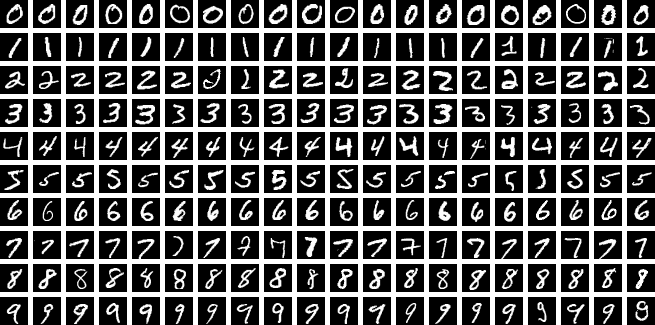
\includegraphics[width=0.7\textwidth]{figures/mnist.png}
    \caption{MNIST dataset example images~\cite{mnistImage}.}
  \end{figure}
\end{frame}

\begin{frame}{Data and Network Structure}
  Model evaluation is done with with 5-fold CV.\\

  \begin{figure}
    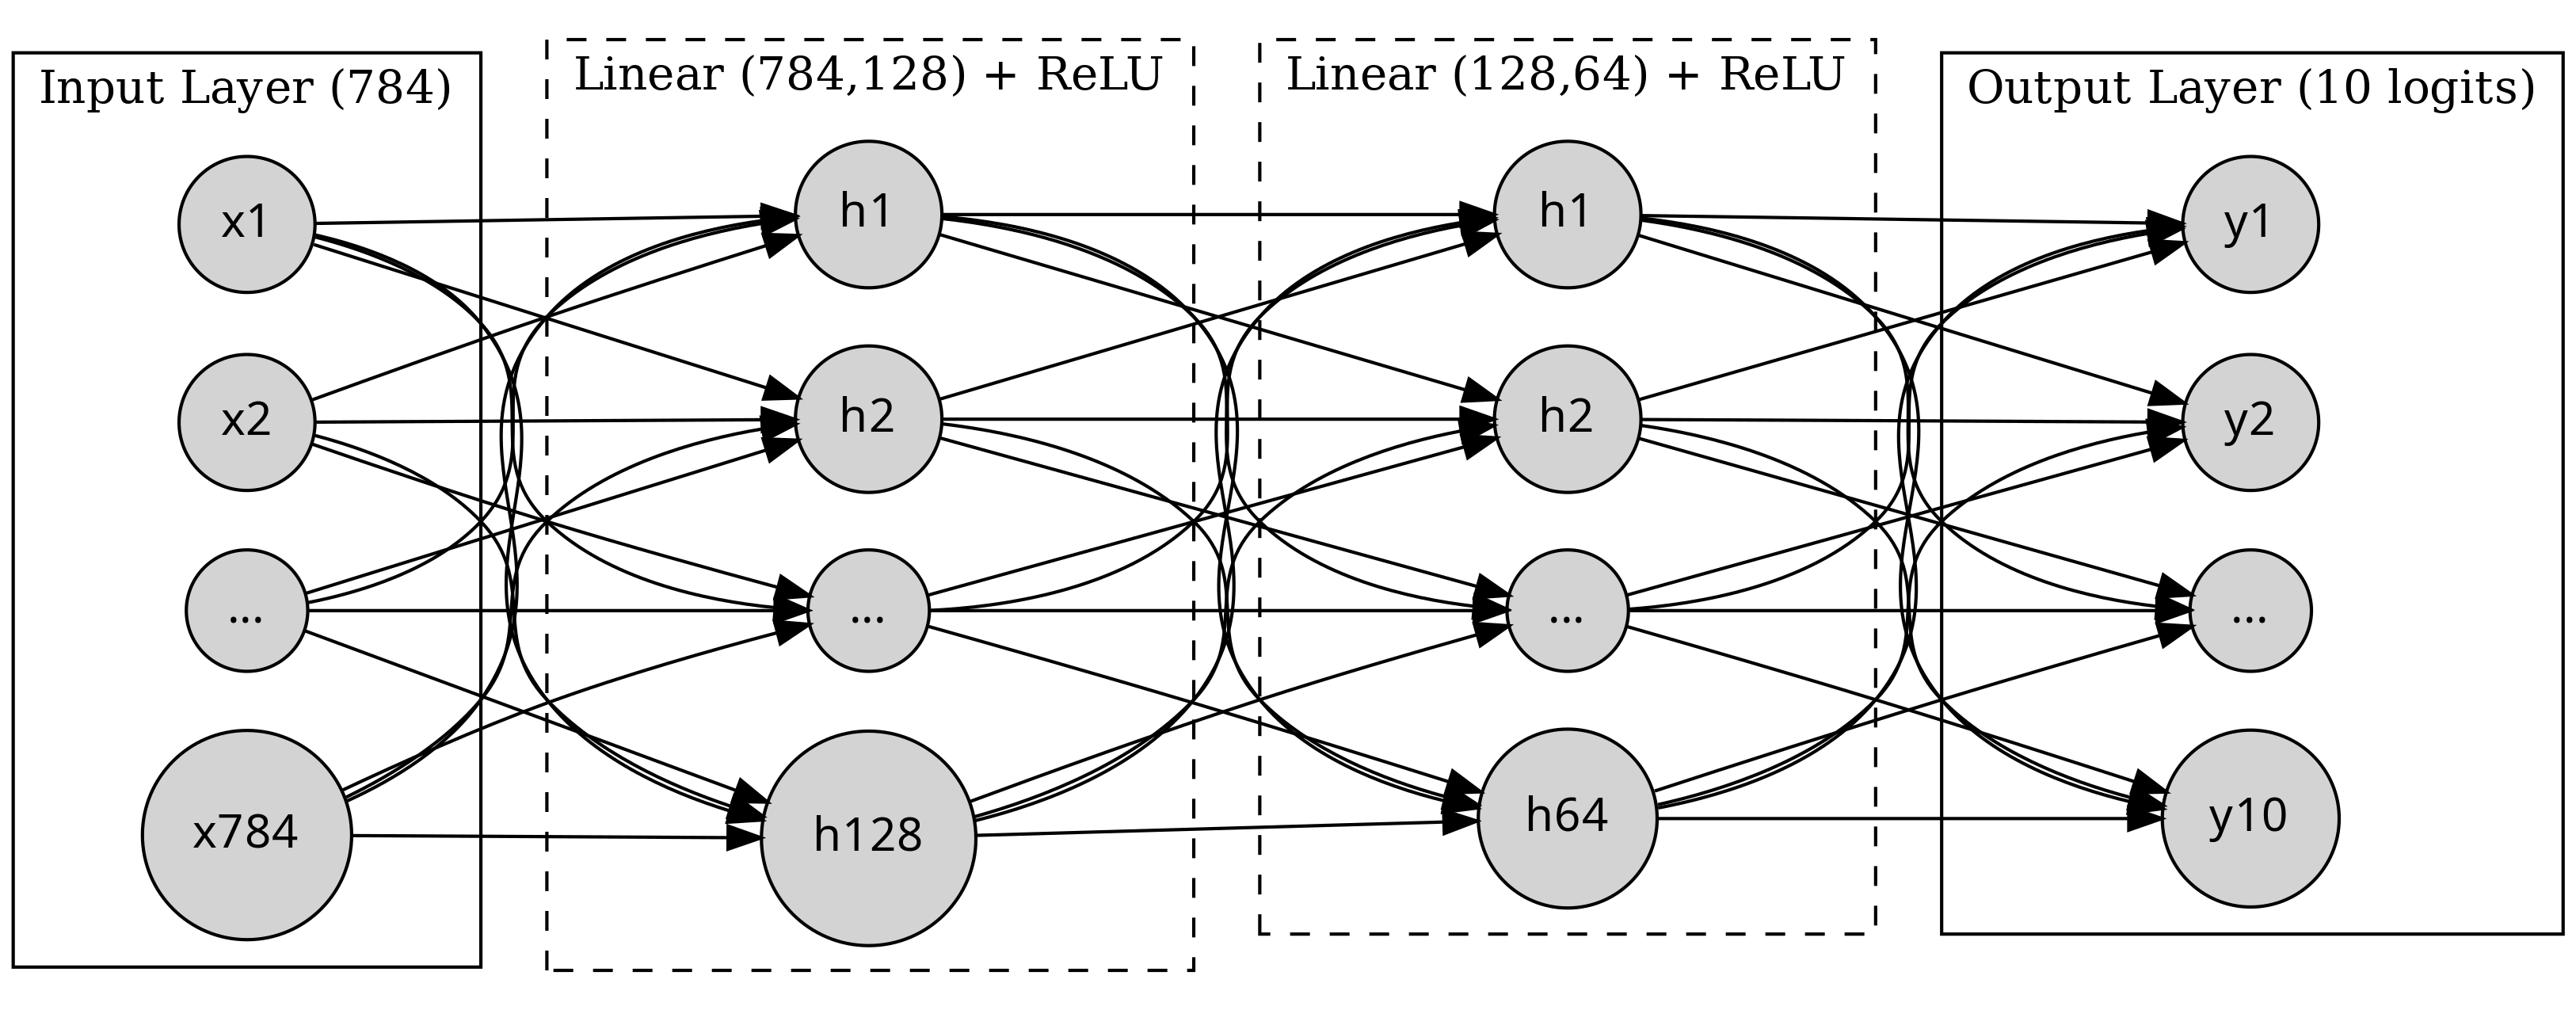
\includegraphics[width=0.8\textwidth]{figures/mlp.png}
    \caption{Structure of simple NN to classify MNIST numbers.}
  \end{figure}
\end{frame}

\begin{frame}{Results - Training and Inference}
  \begin{figure}
    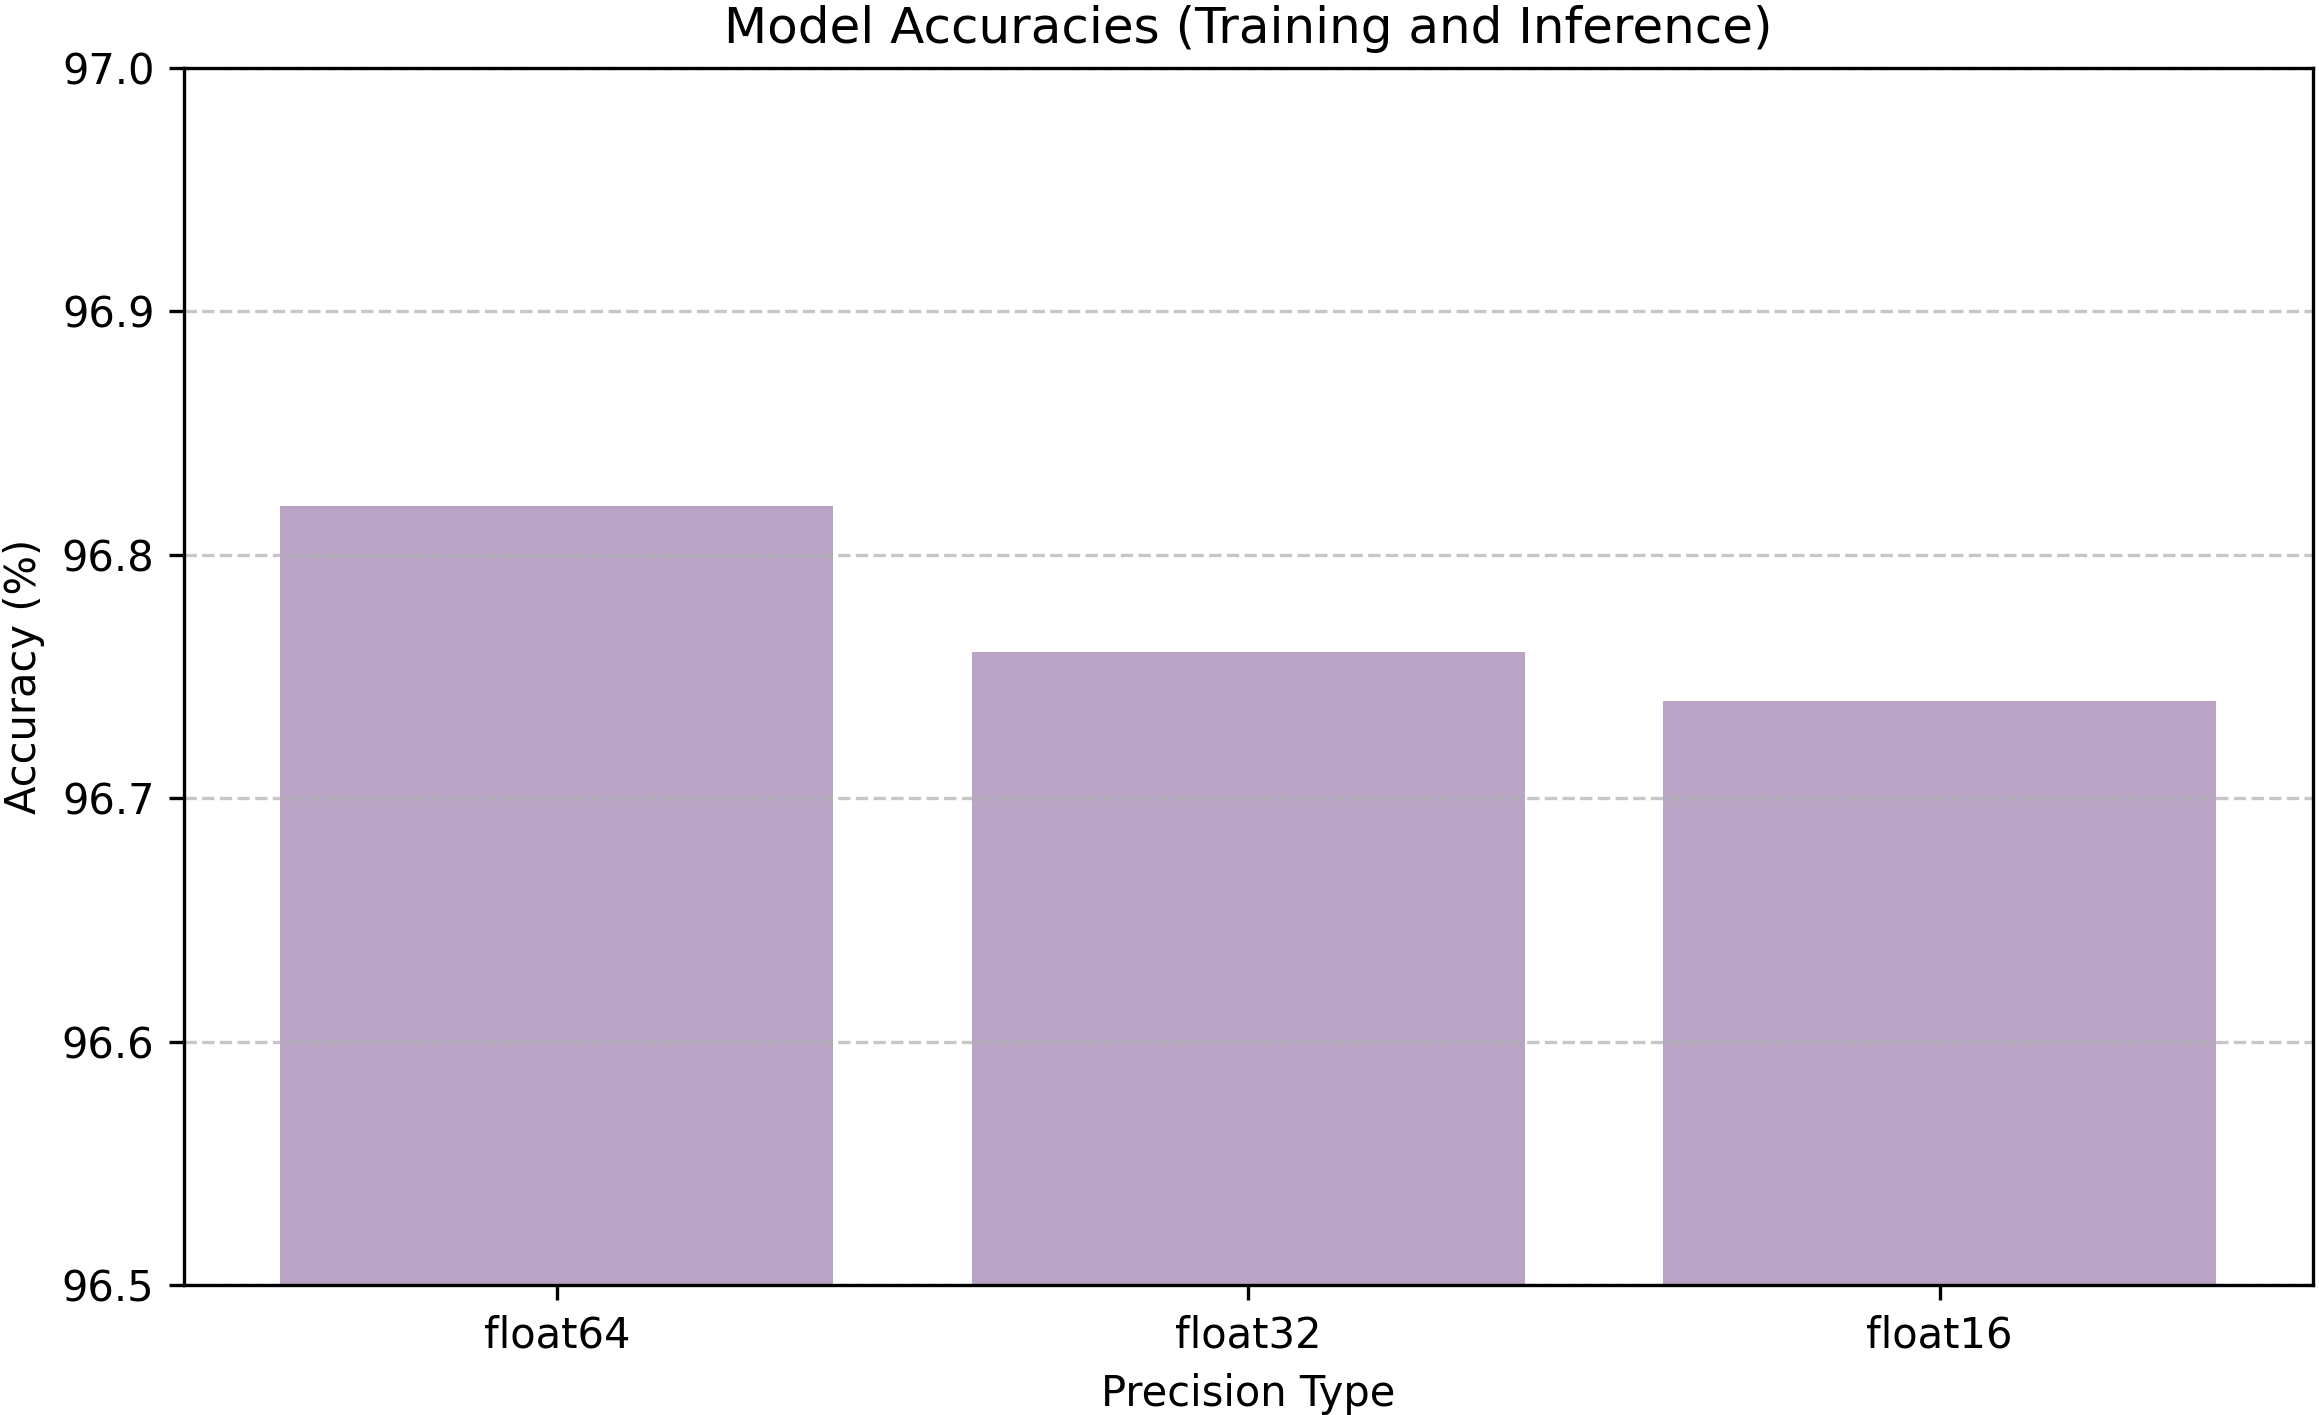
\includegraphics[width=0.7\textwidth]{figures/trainingAndInference.png}
    \caption{Model accuracies - trained and evaluated at each precision.}
  \end{figure}
\end{frame}

\begin{frame}{Results - Training and Inference Times}
  \begin{figure}
    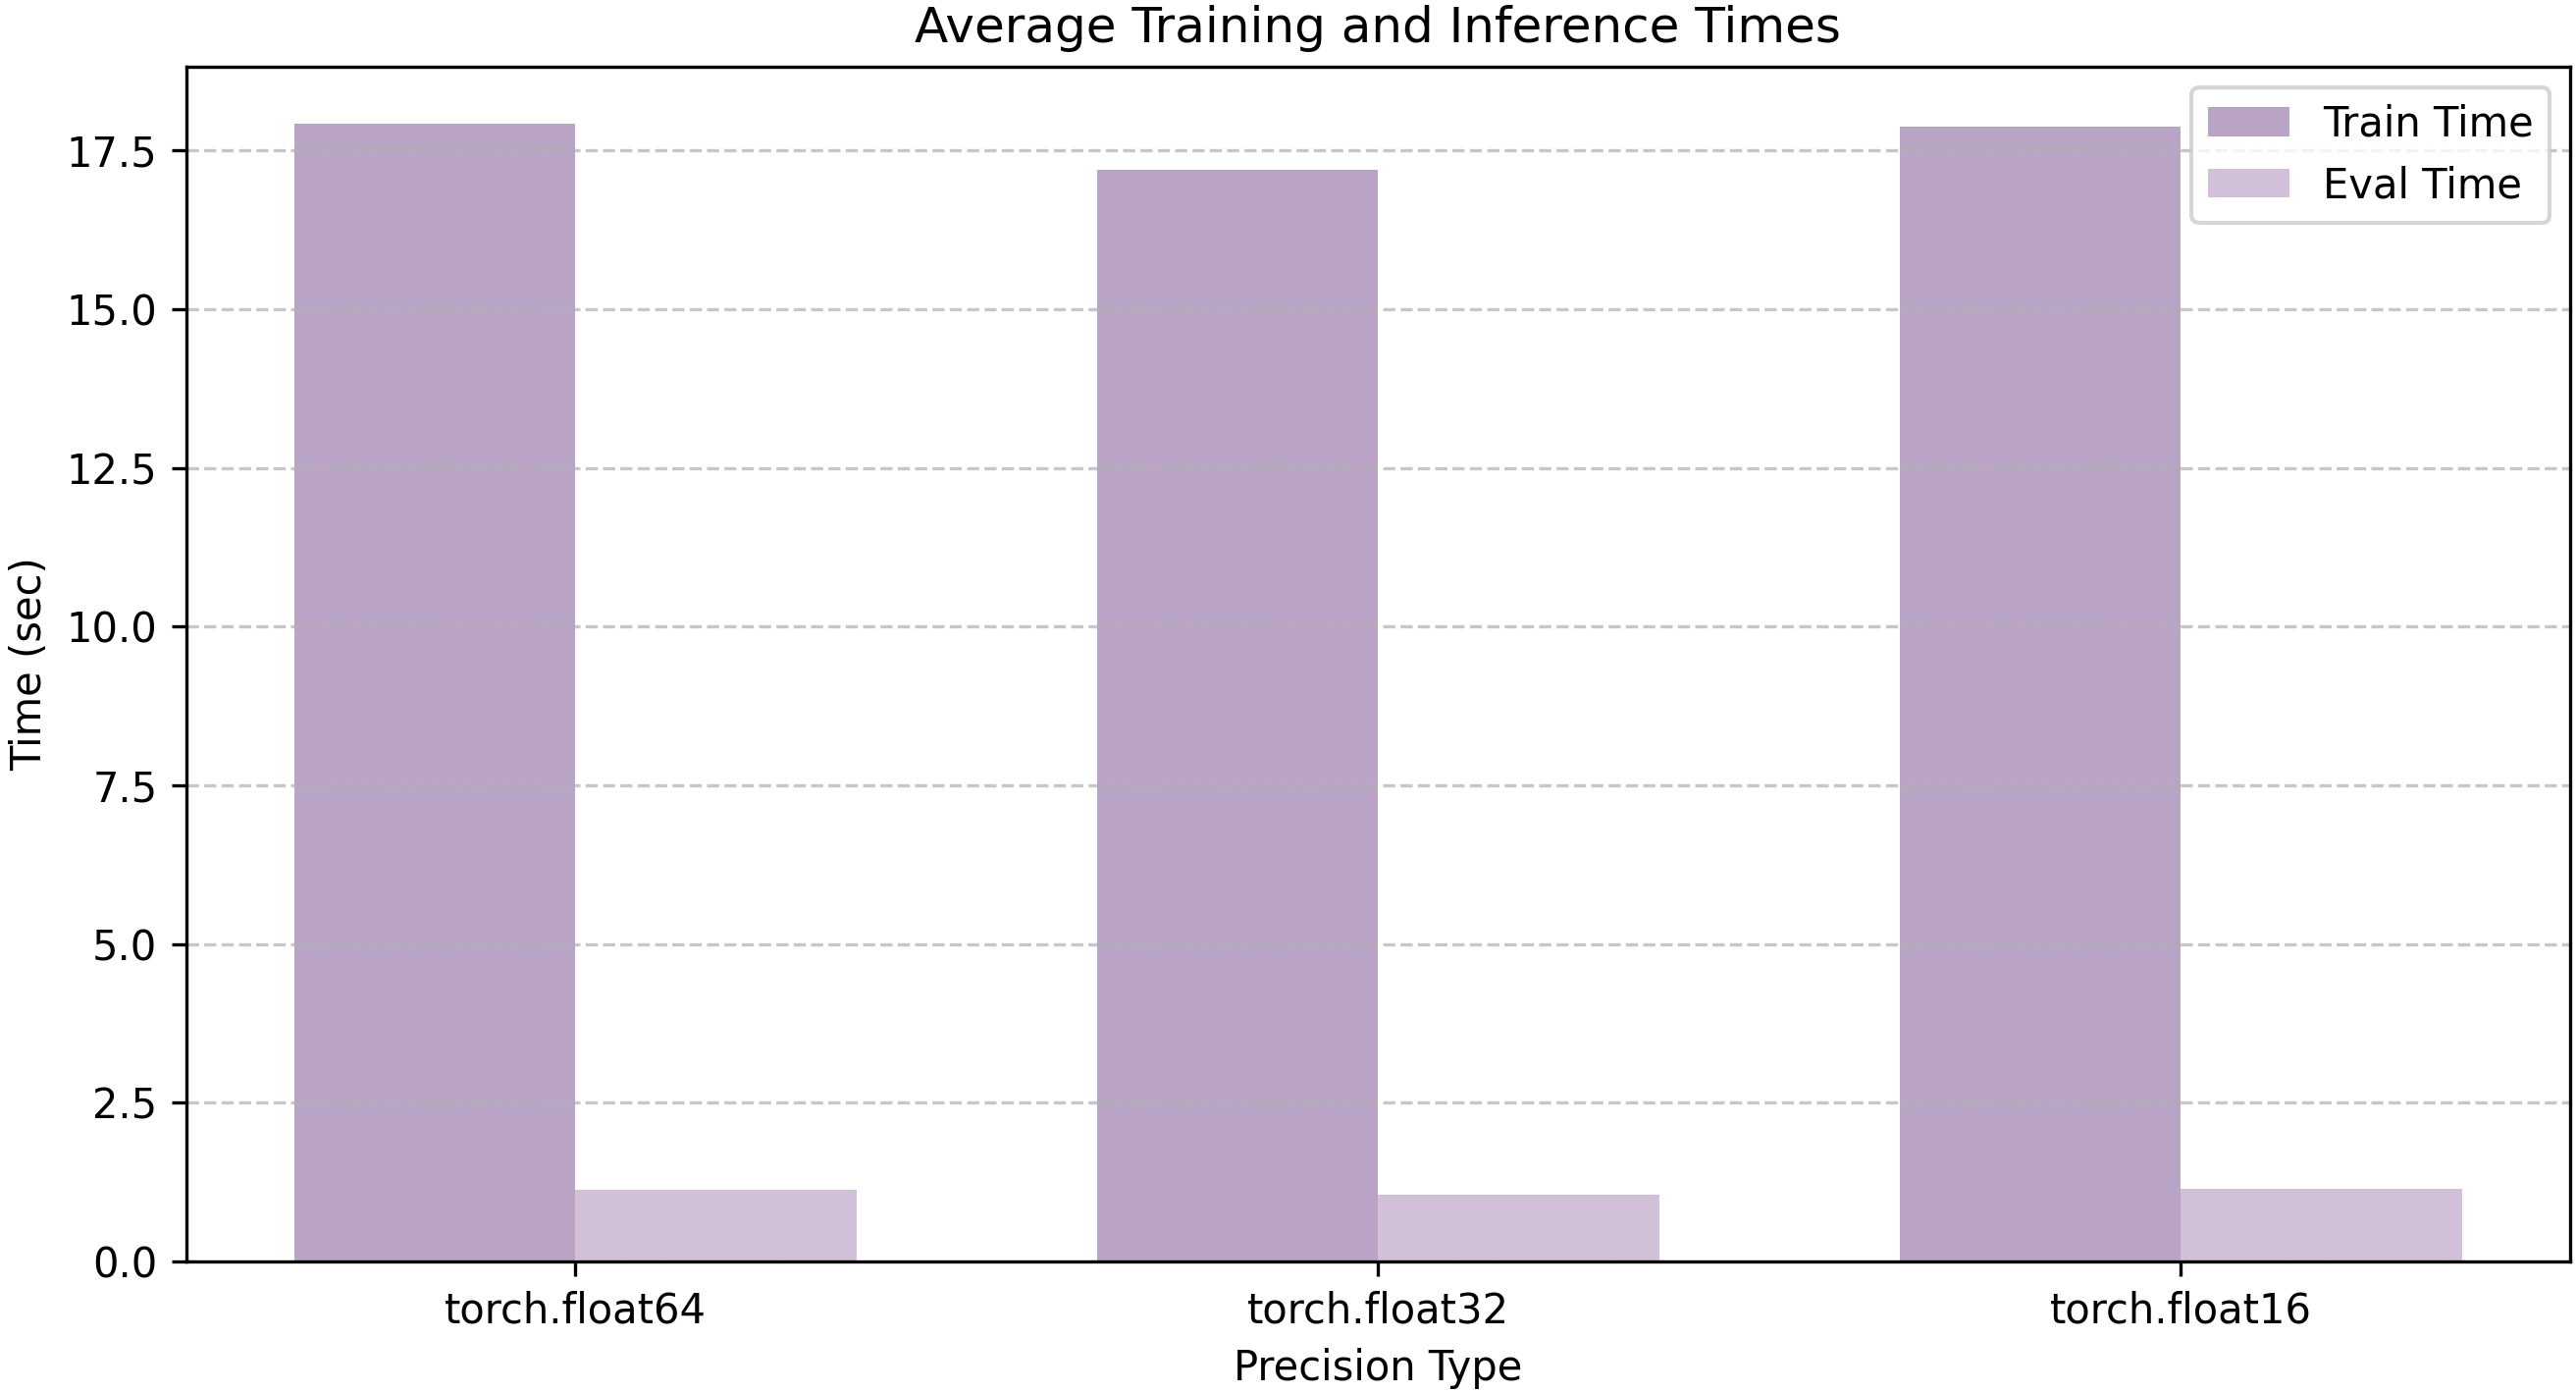
\includegraphics[width=0.7\textwidth]{figures/times.png}
    \caption{Training and evaluation times.}
  \end{figure}
\end{frame}

\begin{frame}{Results - Inference-Only Testing}
  \begin{figure}
    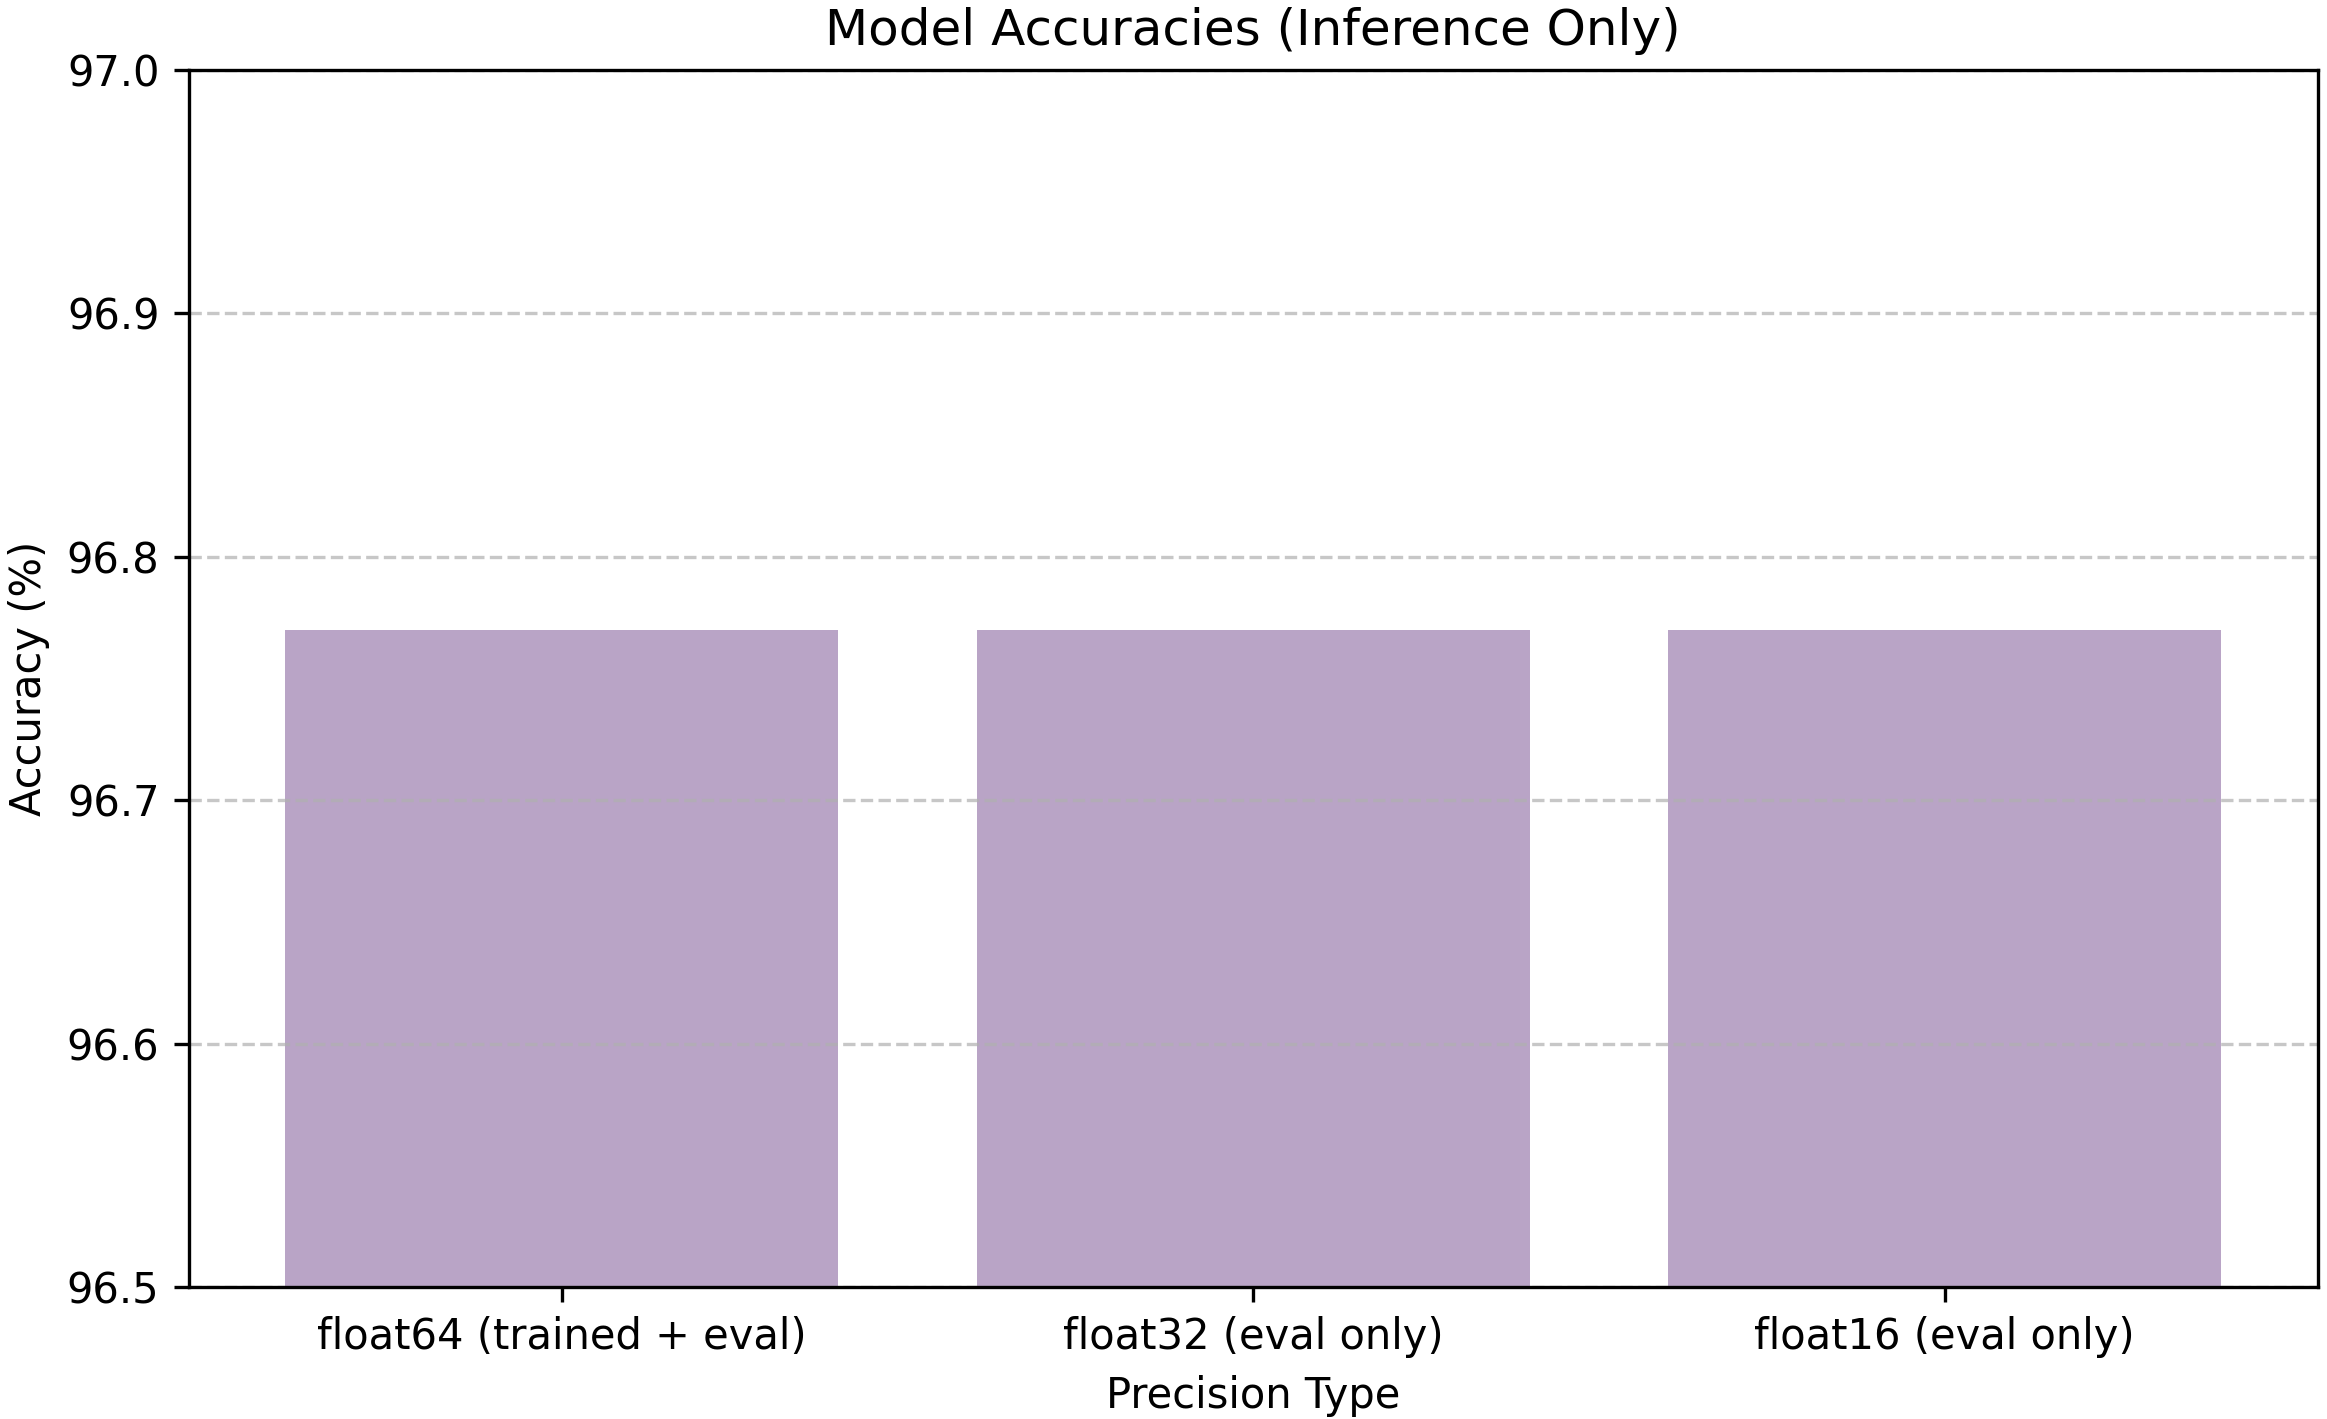
\includegraphics[width=0.7\textwidth]{figures/inferenceOnly.png}
    \caption{Model accuracies - trained with float64 and post-training precision reduction.}
  \end{figure}
\end{frame}

\begin{frame}{Conclusion and Outlook}
  \textbf{Interpretation:} Simple task and simple network $\rightarrow$ almost no effets.\\
  \vspace{0.5cm}
  \textbf{Next Steps:}
  \begin{enumerate}
    \item Reduce precision even further $\rightarrow$ quantize lower than float16 (half
          precision).
    \item Mixed Precision Training $\rightarrow$ different bit-widths for different parts
          of the training process.
  \end{enumerate}
\end{frame}

%%%%%%%%%%%%%%%%%%%%

\begin{skipframecount}
  \begin{frame}[allowframebreaks]{References}
    \printbibliography[heading=none]
  \end{frame}

  \appendix
\end{skipframecount}

\end{document}
